% Working manuscript, revised 2026-11-24.
% Scientific archive: 2025-11-15 through 2026-07-15.
% No observations or production changes after 2026-10-15 are included.
% Figures and quantitative evidence: SHARP commit
% 2f5f71d5a074c4cfd712b0e3fbef240c40745e2a/paper_revision_20261015.
\documentclass[linenumbers]{aastex701}
\usepackage{amsmath}
\usepackage{graphicx}
\usepackage{booktabs}
\usepackage{placeins}
\newcommand{\SHARP}{\textsc{sharp}}
\newcommand{\gaper}{\ensuremath{g_{\rm aper}}}
\newcommand{\asec}{\ensuremath{^{\prime\prime}}}
\newcommand{\degsq}{\ensuremath{\mathrm{deg}^{2}}}
\newcommand{\rateunit}{\ensuremath{\mathrm{arcsec}\,\mathrm{hr}^{-1}}}
\graphicspath{{figures/}}
\shorttitle{The SHARP Ecliptic Small-Body Survey}
\shortauthors{SHARP}
\begin{document}
% Working title; the authors will finalize title, author list, and acknowledgments.
\title{The SHARP Ecliptic Small-Body Survey: Design and Initial Performance}

\begin{abstract}
We present \SHARP, a repeated-imaging survey of the ecliptic with the Xinglong
60/90~cm Schmidt telescope. The survey combines a nominal
$2.94^\circ\times2.95^\circ$ field of view, 30~s exposures, and three planned
visits per field to obtain asteroid astrometry and photometry and to search
for coherent single-night motion. A validated sample from the 2025
November--2026 July initial observing campaign contains 39,590 exposures on 129
observing nights, totaling 329.95~hr of open-shutter time. Their geometric
footprint is $10,928~\degsq$; $10,471~\degsq$ received at least three exposures
within one night during the campaign. The median adjacent-visit interval is
37.65~min, and the median span of sequences with at least three visits is
78.23~min. The median catalog $5\sigma$ model depth is 20.25~mag on the
Gaia-calibrated white-light scale. Within a $1\asec$ association radius,
531,612 positional associations correspond to 58,281 catalog identities,
95.73\% of which lie in the adopted main-belt orbital region; the median
radial observed-minus-computed residual is $0.263\asec$. A retrospective
assessment using the validated exposures gives a conditional linkage
retention of 74.14\% for already-detected known-object nights meeting the
sampling and angular-rate criteria.
The historical motion search yields 58 image-reviewed single-night linkages,
including six consistent with C/2025~Y1 (ATLAS). These results characterize
the delivered coverage, cadence, measurement quality, and linking behavior
of the initial survey and establish its principal use as a source of
repeated asteroid positions and photometry.
\end{abstract}
\keywords{Asteroids (72) --- Sky surveys (1464) --- Astrometry (80) ---
Photometry (1234) --- Time domain astronomy (2109)}

\section{Introduction}
\label{sec:introduction}

Repeated observations of small Solar System bodies provide positions for
orbit determination and photometric measurements of rotational variability.
These uses place different demands on an observing program: an angular
trajectory must be sampled sufficiently to recognize a moving source,
whereas physical characterization benefits from measurements repeated over
longer intervals \citep{WarnerHarrisPravec2009,Denneau2013}. For a wide-field telescope,
the combination of sky coverage, exposure time, and revisit interval
therefore determines which objects can be measured and how the observations
can be used.

Modern surveys illustrate several ways of making these choices. Pan-STARRS
couples wide-field imaging to attribution and linking across multiple
nights; ATLAS emphasizes rapid sky coverage for nearby-object searches;
and the Zwicky Transient Facility (ZTF) combines a large field of view with
repeated imaging for moving-object and time-domain science
\citep{Denneau2013,Tonry2018,Bellm2019,Masci2019}. Dedicated moving-object
processing can also exploit the cadence of a broader time-domain survey,
as demonstrated by the Heliocentric-orbiting Objects Processing System for
the Wide Field Survey Telescope \citep{Wang2025HOPS}. These programs make
clear that sky area, sensitivity, and processing must be considered
together with the temporal sampling actually delivered.

A Schmidt telescope with a moderate aperture and a large field can build a
substantial sample of asteroid measurements through repeated ecliptic
imaging. Its scientific scope is established by the observed footprint,
cadence, and measurement quality, together with the populations represented
on real images. Characterizing these quantities is necessary for selecting
observations suitable for asteroid astrometry, photometric time series,
and moving-source identification.

We developed \SHARP\ for the Xinglong 60/90~cm Schmidt telescope. Its
approximately $2.94^\circ\times2.95^\circ$ field of view is used for repeated
30~s imaging of a predefined ecliptic field library. The observing strategy
aims for three visits to a field during a night, allowing angular motion to
be sampled over roughly an hour. Calibrated source catalogs support two
complementary analyses: association with the predicted positions of known
asteroids and a search for coherent motion among catalog detections. The
initial associated population is dominated by main-belt asteroids, making
their repeated astrometry and photometry the principal initial data product.

Known objects provide a direct way to examine the measurements and
processing. Their predicted positions can be compared with observed
centroids, repeated associations reveal the available time sampling, and
their identities allow stored moving-source linkages to be evaluated on
real detections. The GOTTA Prototype analysis provides a related
application of known-asteroid measurements to survey characterization
\citep[in preparation]{Xiao2026InPrep}. We combine these tests with exposure-level depth
estimates and repeated stellar photometry. The independent motion search
adds an image-reviewed sample of single-night linkages. Linking methods
based on angular trajectories or heliocentric transformations connect such
short arcs to the longer astrometric sequences needed for identification
and orbit determination \citep{Kubica2007,Holman2018,Moeyens2021}.

This paper describes the survey design and its 2025 November--2026 July
initial observing campaign. Section~\ref{sec:survey} introduces the instrument,
photometric convention, observing strategy, and analysis samples.
Section~\ref{sec:processing} describes the moving-object analysis.
Section~\ref{sec:performance} measures the realized footprint, cadence,
photometric and astrometric behavior, and conditional linkage retention.
Section~\ref{sec:samples} presents the associated known-object population
and historical single-night candidates. We discuss the scientific scope
and subsequent use of these measurements in Section~\ref{sec:discussion}
and conclude in Section~\ref{sec:conclusions}.

\section{Survey Design and Data}
\label{sec:survey}

\subsection{Telescope and calibrated measurements}
\label{sec:facility}

\SHARP\ uses the Xinglong 60/90~cm Schmidt telescope, with an effective
aperture of 0.60~m and an $f/3$ optical system. Its camera was developed at
the National Astronomical Observatories, Chinese Academy of Sciences.
The CCD has $9,216\times9,232$ pixels of $10~\mu$m, read through 16
simultaneous output channels. The typical scale is approximately
$1.15\asec$~pixel$^{-1}$, giving a nominal
$2.94^\circ\times2.95^\circ$ field of view. The observatory is listed under
Minor Planet Center (MPC) code 327. Table~\ref{tab:design} summarizes the
parameters used in the initial campaign.

The upstream reduction provides calibrated images (L1) and per-exposure
source catalogs (L2), following bias and flat-field correction, astrometric
solution, source extraction, and photometric calibration
\citep[in preparation]{Li2026InPrep}. Gaia EDR3 provides the astrometric
reference \citep{GaiaEDR32021,Lindegren2021EDR3}. Reference ICRS positions
at catalog epoch J2016.0 are propagated to the Julian year of the UTC
exposure start using the catalog proper motions and Astropy's
\texttt{apply\_space\_motion}, with the right-ascension proper motion
interpreted as $\mu_\alpha\cos\delta$. Parallax and radial velocity are
not supplied; sources with nonfinite propagated coordinates retain their
catalog positions. The propagated coordinates form the reference catalog
consumed by SCAMP, whose fitted TPV solution supplies the final image WCS. The moving-object analysis
begins from these products. The catalogs contain celestial and
image-plane coordinates, observing times, aperture magnitudes and their
uncertainties, and an image World Coordinate System (WCS). The source
measurements use fixed circular apertures in SExtractor
\citep{BertinArnouts1996}. Figure~\ref{fig:exposure} shows a representative image
and four cataloged asteroids.

The initial campaign uses white-light observations, denoted $W$ in the
observing records. The photometric reference is Gaia EDR3
\citep{GaiaEDR32021,Riello2021EDR3}. We retain the
existing notation \gaper\ for the calibrated L2 quantity
\texttt{Mag\_Aper4}: the fourth fixed aperture has a diameter of eight
pixels, or a radius of approximately $4.6\asec$. The symbol refers
throughout this paper to the calibrated white-light magnitude on the
reference scale defined below.

The photometric reference reader also computes propagated coordinates,
but the white-light calibration matches stars using their original
catalog coordinates. The calibration constructs a reference magnitude
from Gaia $G$ and the Gaia color $G_{\rm BP}-G_{\rm RP}$,
\begin{align}
x &= (G_{\rm BP}-G_{\rm RP})-0.340674898,\\
W_{\rm ref} &= G+0.1136777774 + P_W(x),\\
P_W(x) &= -0.03971196x^3+0.19464851x^2
          -0.11042587x-0.03542586.
\label{eq:color}
\end{align}
The per-exposure zero point $ZP$ is determined from an
18-pixel-diameter reference aperture. For a background-subtracted
eight-pixel aperture flux $f_8$ in ADU, the reported magnitude is
\begin{equation}
\gaper = ZP-2.5\log_{10}f_8+C_8,
\label{eq:apercal}
\end{equation}
where $C_8$ is the median difference between the instrumental
18-pixel and eight-pixel aperture magnitudes of the calibration stars.
The corresponding flux correction also scales the flux uncertainty.
This defines the adopted white-light scale; comparisons with predicted
asteroid $V$ magnitudes or standard passbands require color and response
information.

\begin{figure}[tbp]
\centering
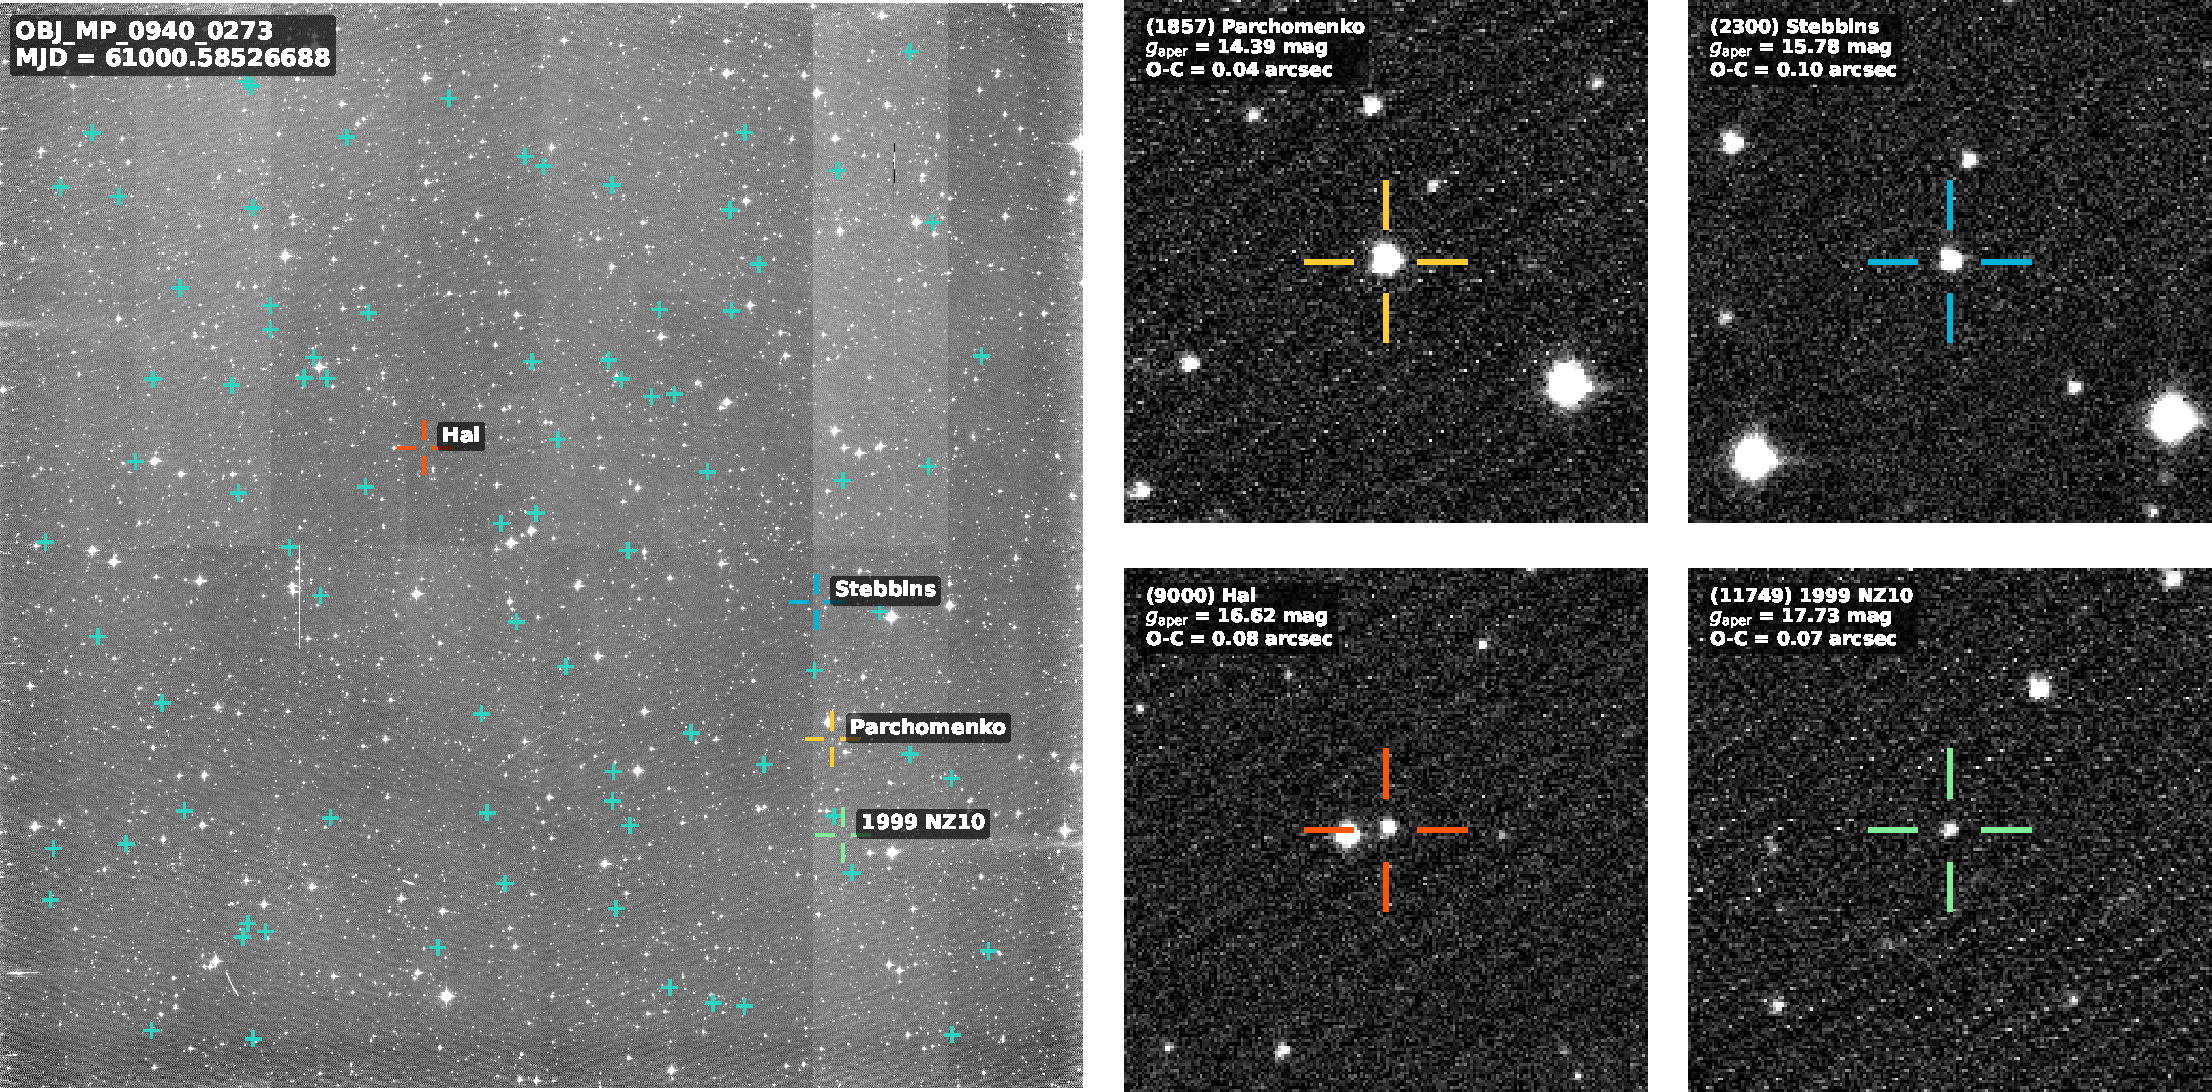
\includegraphics[width=0.98\linewidth]{fig01_exposure.pdf}
\caption{A representative 30~s white-light exposure obtained on 2025
November~21. The wide-field panel marks four known-asteroid associations,
and the four cutouts show their measured positions. Labels give the
calibrated white-light aperture magnitude \gaper\ and the radial
observed-minus-computed (O$-$C) separation within the $1\asec$ association
sample. The displayed MJD is the exposure start time; ephemeris matching
uses the exposure midpoint. The image uses a z-scale display with local
background treatment.}
\label{fig:exposure}
\end{figure}

\begin{table}[tbp]
\centering
\caption{Instrument and Initial Survey Parameters}
\label{tab:design}
\begin{tabular}{ll}
\toprule
Quantity & Value or convention\\
\midrule
Telescope & Xinglong 60/90~cm Schmidt, $f/3$\\
Detector size & $9,216\times9,232$ pixels\\
Pixel size / simultaneous readout channels & $10~\mu$m / 16\\
Typical pixel scale & $\simeq1.15\asec$~pixel$^{-1}$\\
Nominal field of view & $2.94^\circ\times2.95^\circ$\\
Observing band & $W$ (white light)\\
Reported aperture magnitude & Calibrated \texttt{Mag\_Aper4}, denoted \gaper\\
Measurement aperture & Eight-pixel diameter\\
Field library & 1,855 ecliptic fields\\
Standard exposure time & 30~s\\
Nominal visits and interval & Three visits; $\sim30$~min between starts\\
Readout allowance in scheduling & 15~s\\
Minimum planned target altitude & $30^\circ$\\
Known-asteroid prediction limit & $V<22.5$\\
Primary / auxiliary match radii & $1.0\asec$ / $1.5\asec$\\
Independent motion-search window & $3$--$63$~\rateunit\\
\bottomrule
\end{tabular}
\end{table}

\subsection{Observing strategy and analysis sample}
\label{sec:design}

The field library contains 1,855 pointings centered on an ecliptic band,
with field-center ecliptic latitudes from approximately $-18.5^\circ$ to
$+16.3^\circ$. The scheduling design selects observable fields according to
target altitude, seasonal visibility, Moon separation, and stored coverage
history, and groups nearby fields to limit slews. A normal sequence aims
for three visits, with a nominal 30~min interval between repeat starts.
The scheduler includes a 15~s readout allowance in addition to the nominal
30~s exposure and pointing overheads.

The observed footprint and cadence are measured from the actual WCS
pointings and exposure times in Section~\ref{sec:coverage}, encompassing
both completed and partial observing sequences.

\label{sec:cohorts}

The main archive covers 2025 November~15 through 2026 July~15. We select
unique physical exposures with calibrated catalogs, interpretable
exposure times, and usable WCS solutions consistent with the camera
geometry. Repeated files are counted once, and exposures with
inconsistent timing or astrometry are excluded. The selection retains
the range of seeing and photometric conditions in the usable archive;
the supplementary exposure ledger records the individual selections.

For the validated sample, we assign a physical observing night from the
exposure midpoint, with local noon in the Asia/Shanghai time zone as the
boundary. This avoids dividing an observing night at midnight and
resolves some differences from archive-directory labels. The resulting
sample contains 39,590 exposures on 129 physical nights, from 2025
November~16 through 2026 July~15. Its exposure, footprint, photometric,
and known-association statistics form the main performance results.

The linkage assessment compares stored moving-source links with known
identities, both in the original processing sample and after selecting
validated exposures and physical observing nights. The candidate sample
comes from the original image-review record; all 179 measurements in
its 58 retained links map to validated exposures. Their detailed results
are presented in Sections~\ref{sec:retention_results} and
\ref{sec:candidates}.

The scientific inputs and production methods considered in this paper
are restricted to material available by 2026 October~15. All quantitative
survey results refer to the November--July main archive. The archived
configuration and scientific inputs are identified in the data release.

\section{Moving-Object Analysis}
\label{sec:processing}

The calibrated images and catalogs feed the two analysis paths shown in
Figure~\ref{fig:workflow}. Ephemeris association measures sources at
predicted asteroid positions. The independent search first seeks
consistent motion, then uses the known-object associations to remove
already attributed linkages. Both paths retain the connection between a
measurement, its exposure, and the corresponding image.

\begin{figure}[tbp]
\centering
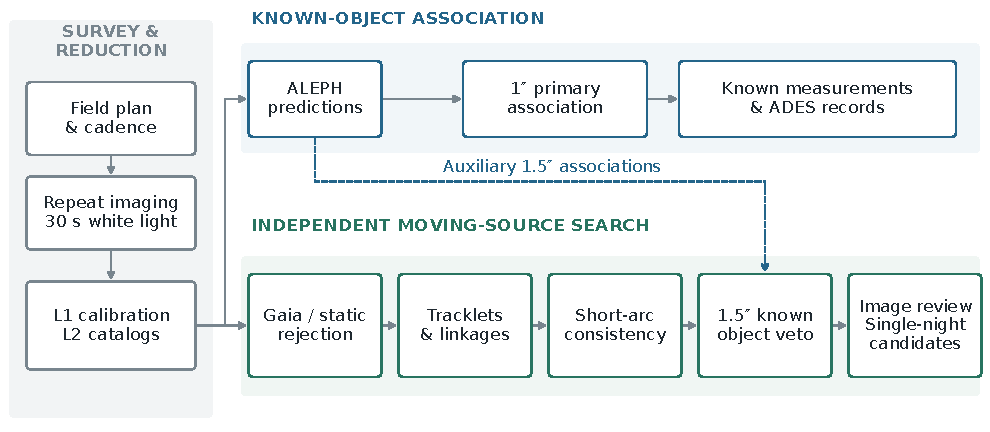
\includegraphics[width=\linewidth]{fig02_workflow.pdf}
\caption{The observing and analysis sequence used in the initial \SHARP\
campaign. Repeated white-light imaging produces calibrated L1 images
and L2 source catalogs. The upper branch associates measured sources
with ALEPH predictions and supplies the primary $1\asec$ known-object
sample. The independent moving-source branch constructs tracklets and
links after static-source rejection, tests short-arc consistency, and
then removes links identified through auxiliary $1.5\asec$ known-object
associations. The dashed connection supplies these identities after
moving-source linking. Image review selects the retained single-night
candidates.}
\label{fig:workflow}
\end{figure}

\label{sec:known_method}

For each exposure, the known-object branch evaluates topocentric asteroid
directions at the exposure midpoint using the archived Lowell
\texttt{astorb} orbital catalog \citep{Moskovitz2022Astorb} and
ALEPH version~1.0.0 \citep{PenaZamudioFuentes2021ALEPH}. The prediction uses the
Xinglong position adopted by the historical matcher:
$117.575^\circ$ east longitude, $40.393^\circ$ north latitude, and 960~m
height. We use this location consistently for the known-object
viewing geometry.

Predictions with $V<22.5$ that fall within the image geometry are compared
with measured sources. The primary catalog retains the nearest
association within $1.0\asec$; a separate $1.5\asec$ association table is
used for known-object subtraction and processing diagnostics. The
predicted magnitude limit defines the ephemeris query, rather than the
exposure detection limit. The historical matcher checks finite
photometric fields but does not impose a physically restrictive
consistency cut between predicted $V$ and measured \gaper. This matters
particularly for sparse associations to objects in less populated
orbital regions.

The prediction catalog contains asteroid orbital elements. Comets were
therefore outside the contemporaneous known-object subtraction, a point
relevant to the C/2025~Y1 associations discussed in
Section~\ref{sec:candidates}. Selected measurements are also stored in
Astrometric Data Exchange Standard (ADES) format.

\label{sec:motion_method}

The independent search starts from detections in repeated catalogs of a
field. Gaia associations, stationary-source patterns, and edge-related
detections are removed before constructing two-detection tracklets.
Tracklets sharing endpoints can be combined into links with at least
three measurements. The historical search accepts angular rates of
$3$--$63$~\rateunit, a magnitude difference no larger than 1~mag within
a tracklet, a tracklet-rate difference no larger than
5~\rateunit, and a direction difference no larger than $10^\circ$.
These criteria define the initial search window and help suppress
inconsistent combinations of detections.

A heliocentric short-arc calculation then tests whether a candidate chain
admits a consistent trajectory. Heliocentric transformations are useful
for linking moving-source observations \citep{Holman2018}; the
implementation used here evaluates the within-night chains generated by
the preceding tracklet step. A successful short-arc fit and the absence
of auxiliary known-asteroid associations for all members define the
historical automatic candidate catalog. All 4,762 selected links also satisfy the separately evaluated
diagnostic thresholds: fit RMS $\leq5\asec$, maximum residual
$\leq8\asec$, and linear-trajectory RMS $\leq10\asec$.

The short-arc calculation solves a solar two-body Lambert problem
\citep{Izzo2015}, using eight equal-endpoint heliocentric-distance
hypotheses, $r=1.3,1.7,\ldots,4.1$~au. It compares the angular
RMS of solutions for the full chain and tracklet subsets, with
observer distances greater than 0.02~au at both endpoints and
a final-epoch heliocentric speed below 35~km~s$^{-1}$ for
accepted fits. The discrete distance hypotheses construct the
Lambert endpoints; they are not a constraint on the fitted
semimajor axis. Further implementation details are given in
Appendix~\ref{app:shortarc}.

The surviving links are displayed as time-ordered image sequences for
visual review. The review checks source morphology, blending, artifacts,
and whether the observed displacement is consistent across the images.
The preserved review record distinguishes automatic links, initial
positive review, submission selection, and the sample retained after
further image checks. We use the last of these for the candidate
description in Section~\ref{sec:candidates}.

\label{sec:retention_method}

Known identities in the $1.5\asec$ auxiliary association table provide a
retrospective test of the stored motion-search links. An eligible
object--night has at least three detected associations and a predicted
first-to-last angular rate within $3$--$63$~\rateunit. It is retained if
an existing link contains at least three detections, all of which map
to that known identity. Ambiguous identity assignments are excluded from this mapping.

We define the conditional retention as
\begin{equation}
R_{\rm cond} =
\frac{N_{\rm eligible\ object\text{--}nights\ represented\ by\ a\ link}}
     {N_{\rm eligible\ detected\ object\text{--}nights}}.
\label{eq:retention}
\end{equation}
The links are assessed before known-object subtraction so that
successfully linked known asteroids can be counted. The denominator
already requires catalog detections and suitable sampling. Thus this
test measures the assembly of available detections into links, not the
probability that an arbitrary asteroid entering the images is detected.

Figure~\ref{fig:retention} uses the original processing cohort.
We also reconstruct the eligible sample using validated exposures,
distinct physical exposure identifiers, and physical observing nights.
This reconstruction applies the same rate and minimum-sampling criteria
and tests membership in the existing pre-subtraction links.
The measured retention combines field grouping, source filtering,
tracklet construction, and short-arc screening. Stage-specific
processing states are recorded in the supplementary tables.

\section{Observing Performance}
\label{sec:performance}

\subsection{Realized footprint and cadence}
\label{sec:coverage}

The 39,590 validated exposures correspond to 329.95~hr of open-shutter
time. This is the sum of exposure durations, excluding readout,
slews, and other overheads. Table~\ref{tab:results} collects the principal
performance measurements and identifies their statistical samples.

We derive each footprint from the corners of its verified L2 image
WCS, including the archived TPV distortion solution. Overlaps are
combined on a HEALPix grid \citep{Gorski2005}, using a pixel-center
test for membership in each footprint polygon. The area covered at
least once is $10,928.1~\degsq$. A second measure first counts visits
within each physical observing night and then takes the union of
sky pixels receiving at least three exposures on any one night;
this area is $10,470.6~\degsq$. The adopted totals use $N_{\rm side}=1024$ and measure the geometric
footprint of the validated exposures.

Figure~\ref{fig:coverage} compares the accumulated exposure coverage
with the spatial distribution of the known-object associations.
Both show the ecliptic observing region, but the quantities have
different weightings. Exposure density measures where the camera
observed, whereas association density also depends on the population,
geometry, sensitivity, and catalog selection. The footprint uses the actual WCS pointings.

\begin{figure}[tbp]
\centering
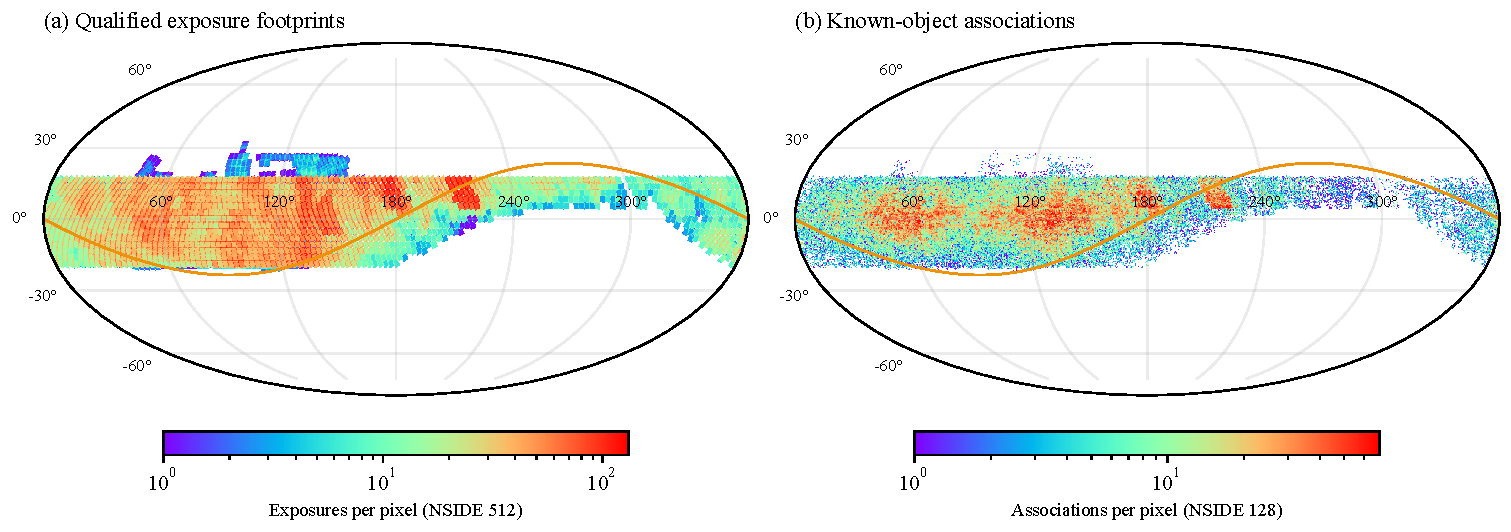
\includegraphics[width=\linewidth]{fig03_coverage_and_known_sky.pdf}
\caption{The accumulated \SHARP\ observations in J2000 ecliptic
longitude and latitude. (a) Number of validated exposures covering
each HEALPix pixel, using actual image WCS footprints and
$N_{\rm side}=512$. (b) Number of primary $1\asec$ known-object
associations per pixel at $N_{\rm side}=128$. The orange curve is
the celestial equator. The color scales are logarithmic and
represent different statistical units and pixel areas. The
geometric areas quoted in the text are evaluated at
$N_{\rm side}=1024$.}
\label{fig:coverage}
\end{figure}

To measure the within-night cadence, we group exposures by physical
observing night, recorded field identifier, and actual WCS pointing.
Complete-link grouping requires any two centers in a group to be
separated by at most $0.30^\circ$, approximately one tenth of the
camera width, so that images with substantially different pointings
are assigned to separate observing sequences.

The resulting 14,400 field--night pointing groups contain 2,651
single visits, 2,039 pairs, and 9,710 sequences with at least three
visits. Thus 67.43\% of groups supply three or more validated
exposures. The median interval among the 25,190 adjacent
exposure pairs is 37.65~min, with a 16th--84th percentile range of
28.37--41.92~min. For the groups with at least three visits, the
median first-to-last span is 78.23~min, with a corresponding range
of 61.93--91.50~min.

Figure~\ref{fig:cadence} shows the observing activity and cadence
distributions. The observed spacing is longer than the nominal
30~min design value, and the distributions include incomplete and
extended sequences. The cumulative area that has ever received
three within-night exposures and the fraction of individual
field--night groups completing three visits answer different
questions; both are needed to describe the sampling available
for moving-source searches.

\begin{figure}[tbp]
\centering
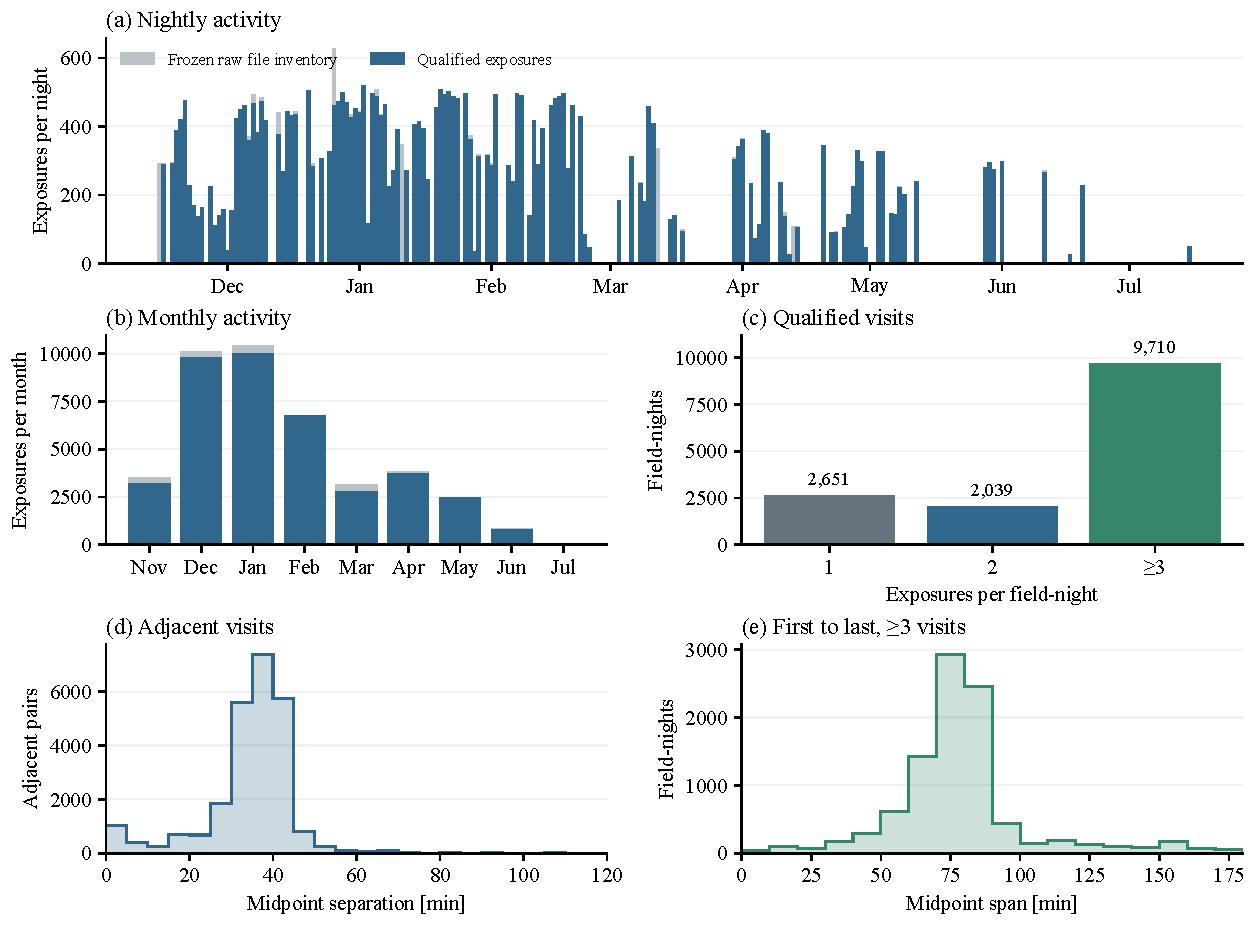
\includegraphics[width=0.96\linewidth]{fig04_activity_and_cadence.pdf}
\caption{Observing activity and realized cadence. (a,b) Nightly
and monthly counts in the original raw-file inventory and the
validated exposure sample. Both counts in (a,b) are grouped by
archive-directory date for a direct inventory comparison.
Panels (c--e) use exposure midpoints and local-noon observing
nights. (c) Number of validated visits in each of the
14,400 field--night pointing groups. (d) Midpoint separation of
25,190 adjacent exposure pairs within those groups. (e)
First-to-last midpoint span for the 9,710 groups containing at
least three visits. The plotted interval ranges emphasize the
main distributions; the accompanying machine-readable histograms
retain the full tails.}
\label{fig:cadence}
\end{figure}

\begin{table}[tbp]
\centering
\caption{Principal Measurements of the Initial Campaign}
\label{tab:results}
\begin{tabular}{ll}
\toprule
Quantity & Measured value\\
\midrule
\multicolumn{2}{l}{\textit{Validated exposure sample}}\\
Exposures / physical observing nights & 39,590 / 129\\
Open-shutter time & 329.95~hr\\
Geometric area with at least one exposure & $10,928.1~\degsq$\\
Area ever reaching three exposures in one night & $10,470.6~\degsq$\\
Field--night groups with at least three visits & 9,710 / 14,400 (67.43\%)\\
Median adjacent-visit interval & 37.65~min\\
Median span of sequences with at least three visits & 78.23~min\\
Median catalog $5\sigma$ model depth & 20.25~mag\\
Model-depth interquartile range & 19.76--20.58~mag\\
\midrule
\multicolumn{2}{l}{\textit{Primary $1\asec$ associations in validated exposures}}\\
Associations / catalog identities & 531,612 / 58,281\\
Identities in the main-belt orbital region & 55,791 (95.73\%)\\
Median radial O$-$C separation & $0.263\asec$\\
Robust scatter in $\Delta\alpha\cos\delta$ / $\Delta\delta$ & $0.222\asec$ / $0.215\asec$\\
\midrule
\multicolumn{2}{l}{\textit{Linkage assessment and reviewed candidates}}\\
Historical conditional retention & 75,899 / 102,347 (74.16\%)\\
After exposure and night validation & 75,467 / 101,784 (74.14\%)\\
Image-reviewed single-night linkages & 58\\
Measurements / nights in retained linkages & 179 / 34\\
\bottomrule
\end{tabular}
\tablecomments{Model depth is defined by Equation~\ref{eq:depth}.
Astrometric scatter is $0.7413\,\mathrm{IQR}$ within the primary
association selection. The two retention rows use the cohorts defined in
Section~\ref{sec:retention_results}. All 179 reviewed candidate
measurements belong to validated exposures.}
\end{table}

\subsection{Photometric and astrometric performance}
\label{sec:photometry}

The validated images have a median catalog image FWHM of
$3.58\asec$, with an interquartile range of
$3.16$--$4.24\asec$. The per-exposure depth summary uses the
archived L2 quantity \texttt{MLIM}. Its calculation is
\begin{align}
F_{5,\rm ADU} &=
\frac{5}{g_{\rm e}}\left[(s_{\rm ADU}g_{\rm e}+r_{\rm e}^{\,2})
                 \,\pi\left(\frac{w_{\rm pix}}{2}\right)^2
                 \right]^{1/2},\\
m_{5,\rm model} &= ZP-2.5\log_{10} F_{5,\rm ADU},
\label{eq:depth}
\end{align}
where $s_{\rm ADU}$ is the sky level per pixel, $g_{\rm e}$ is
the gain in electrons per ADU, $r_{\rm e}$ is the read noise in
electrons, $w_{\rm pix}$ is the image FWHM in pixels, and $ZP$
is the exposure's zero point for the 18-pixel-diameter reference
aperture. This background-plus-read-noise model uses a circular noise
area with radius FWHM/2. It applies no separate encircled-energy
correction at that radius and does not use the eight-pixel aperture
correction in Equation~\ref{eq:apercal}.

The median model depth is 20.25~mag, and the interquartile range
is 19.76--20.58~mag (Figure~\ref{fig:quality}a). Its noise
aperture differs from the fixed eight-pixel-diameter aperture used for
\gaper. We therefore report this value specifically as the catalog
background-noise model depth.

Figure~\ref{fig:quality}b shows the cataloged aperture-magnitude
uncertainties of unflagged known-object associations with positive
aperture fluxes and errors. An independent
short-timescale check uses 18 archived L2 catalogs in six selected
field--night sequences. We match isolated, unflagged, stellar
detections between visits and estimate a per-epoch scatter from
their magnitude differences,
\begin{equation}
\sigma_{\rm epoch} =
\frac{0.7413\,\mathrm{IQR}(\Delta g_{\rm aper})}{\sqrt{2}}.
\label{eq:repeatability}
\end{equation}
This estimator converts the interquartile spread to a
Gaussian-equivalent scatter and attributes comparable noise
to the two epochs.

At $15.5\leq\gaper<16$, the estimated scatter is 0.0118~mag,
compared with a median reported uncertainty of 0.0115~mag.
At $17.5\leq\gaper<18$, the corresponding values are
0.0569 and 0.0574~mag. The agreement supports the short-timescale
precision of the aperture measurements for these selected
conditions. The sequences preferentially sample cleaner images,
and the stars have not been screened independently for
long-term variability; this check is consequently limited to
within-night repeatability.

\label{sec:astrometry}

For each primary association we form observed-minus-computed
residuals in right ascension and declination. The right-ascension
difference is wrapped into the interval $[-180^\circ,180^\circ]$
and multiplied by the cosine of the predicted declination.
The 531,612 primary associations have a median radial
separation of $0.263\asec$. The median components are
$-0.0167\asec$ in $\Delta\alpha\cos\delta$ and
$+0.0224\asec$ in $\Delta\delta$, with
$0.7413\,\mathrm{IQR}$ scatters of $0.2215\asec$ and
$0.2152\asec$, respectively.

Figure~\ref{fig:quality}c shows the magnitude dependence of the
radial residuals. They are smallest at intermediate brightness and
increase toward both ends of the plotted range. Panel~(d) shows
nightly medians of the signed components and the number of
associations supporting each night. Nightly shifts remain visible
even when the pooled component medians are close to zero. These diagnostics
describe the combined image measurement, reference-frame,
timing, and ephemeris agreement of the selected associations.
The $1\asec$ matching radius truncates the distribution.
For comparison, the auxiliary $1.5\asec$ sample contains
560,127 associations and has a median radial residual of
$0.277\asec$; 28,515 of those associations lie between
$1.0\asec$ and $1.5\asec$.

\begin{figure}[tbp]
\centering
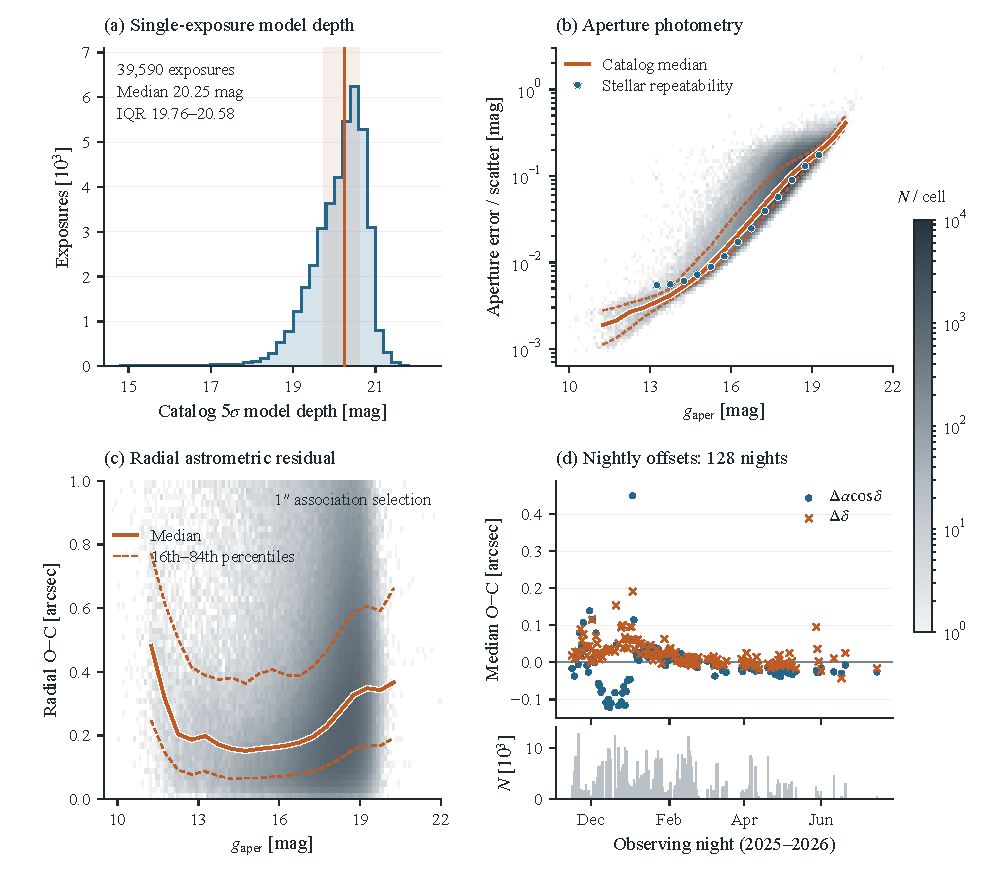
\includegraphics[width=\linewidth]{fig05_measurement_quality.pdf}
\caption{Measurement quality in the validated exposure sample.
(a) Catalog $5\sigma$ model depth for 39,590 exposures in 0.2-mag bins;
the orange line and shaded band mark the median and interquartile range.
(b) Reported aperture error for 500,092 unflagged primary associations
with positive magnitude error, flux, and flux error. Counts use
0.1-mag by 0.04-dex cells. In (b,c), solid and dashed orange curves show
the median and 16th--84th percentiles in 0.5-mag bins containing at least
30 measurements. Blue points in (b) show the stellar repeatability of
Equation~\ref{eq:repeatability} for the six selected field--night
sequences, using bins with at least 50 stellar pairs.
(c) Great-circle radial O$-$C separation, in 0.1-mag by $0.02\asec$
cells. The displayed magnitude range contains 531,416 of the 531,612
primary associations; 195 entries with placeholder magnitude 99 and
one entry at 23.18~mag fall outside it. The shared logarithmic color
bar gives counts per plotted cell. The astrometric distribution is
selected within $1\asec$.
(d) Nightly medians of the signed residuals for all 531,612
associations over 128 physical observing nights; the lower gray
bars give the number of associations in each night. The symbol
\gaper\ denotes the white-light scale defined in
Section~\ref{sec:facility}.}
\label{fig:quality}
\end{figure}

\subsection{Retention of already-detected known-object nights}
\label{sec:retention_results}

Applying the historical definition in
Section~\ref{sec:retention_method} gives 75,899 retained
object--nights out of 102,347 eligible detected
object--nights, or $R_{\rm cond}=74.16\%$. The formal
95\% Wilson interval is 73.89--74.43\%. This interval
summarizes binomial counting uncertainty for the specified
cohort; it does not include correlations among nights or
uncertainty in the sample selection.

Figure~\ref{fig:retention} resolves the result in median
object--night \gaper\ and predicted first-to-last angular rate.
The count map shows where the eligible sample constrains this test,
and the adjacent map gives the retained fraction in the same cells.
The one-dimensional panels summarize the marginal behavior with
their corresponding sample counts. The lowest-rate bin, $3$--$5$~\rateunit,
retains 566 of 1,400 object--nights (40.43\%). The
brightest bin, $10\leq\gaper<13$, retains 262 of 643
(40.75\%). The loss at these edges shows why a single
aggregate fraction does not fully describe the processing.
Source filtering, available displacements, sampling,
and the composition of each detected subset all enter
the result.

Reconstructing the eligible object--night sample from validated
exposures and physical observing nights gives 75,467 linked
object--nights out of 101,784 (74.14\%) over 126 nights.
This calculation reuses the original pre-subtraction links and
retains the historical processing-state policy. Restricting the same
selection to nonquarantined nights with readable stage products gives
73,787/99,426 (74.21\%) over 122 nights. The close agreement with
74.16\% shows that the aggregate result changes little after
exposure and time reconciliation; the three sample definitions are
preserved separately in the accompanying tables.

\begin{figure}[tbp]
\centering
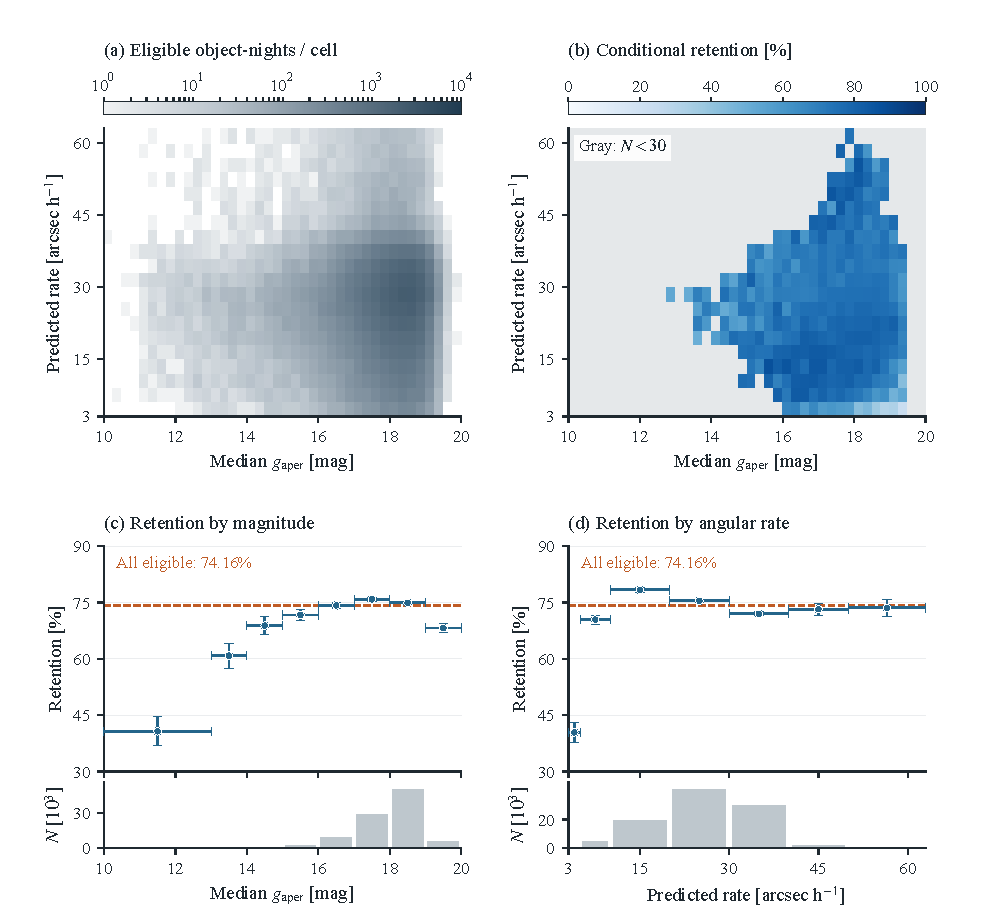
\includegraphics[width=\linewidth]{fig06_conditional_retention.pdf}
\caption{Conditional linkage retention in the historical object--night
sample. Eligibility requires at least three detections associated
with one identity within $1.5\asec$ and a predicted first-to-last
rate of $3$--$63$~\rateunit. A retained object--night is represented
by an existing link with at least three members mapping to that
identity. (a) Eligible counts in 0.25-mag by
3~\rateunit\ cells, on a logarithmic color scale.
(b) Retained fractions in the same cells; cells with fewer than
30 eligible object--nights are masked in gray.
(c,d) One-dimensional retained fractions with 95\% Wilson intervals
and horizontal bars spanning the bins. The lower histograms show
eligible counts per bin. The dashed line is the full historical
fraction, 75,899/102,347 (74.16\%).
The magnitude-dependent panels (a--c) contain 102,315 eligible
object--nights and 75,897 retained cases. They omit 32 object--nights
with unusable magnitudes, including two retained cases, which remain
in the overall and rate-dependent samples. Both two-dimensional
maps use unsmoothed counts. These panels retain the original
processing cohort; the exposure-validated comparison is given in
the text.}
\label{fig:retention}
\end{figure}

\section{Initial Asteroid Results}
\label{sec:samples}

\subsection{The associated known-object population}
\label{sec:known_population}

The primary $1\asec$ sample contains 531,612 associations to
58,281 catalog identities on 128 physical observing nights.
Figure~\ref{fig:orbits} shows the cataloged orbital elements once
per identity, together with the number of observing nights and
the first-to-last measurement span. Counting identities once
separates the population represented in the catalog from the
detection-weighted sky map in Figure~\ref{fig:coverage}.

The adopted main-belt region contains 55,791 identities,
or 95.73\% of the sample. Other points occupy the inner-belt,
Mars-crossing, outer-belt, Jupiter Trojan, near-Earth, and
distant-orbit regions. Here the near-Earth label uses
$q<1.3$~au, while the distant label uses the broad cut
$a\geq5.4$~au. The Jupiter Trojan label denotes a
semimajor-axis region, not a resonance classification
derived in this work.

We examine the 119 positional associations to 17 catalog identities
in the distant-orbit region using neighboring exposures and local
image cutouts. Comparing a stationary-source hypothesis with the
predicted displacement supports motion for 79 associations belonging
to seven identities and identifies nine stationary-source
coincidences belonging to seven other identities. The remaining
31 associations lack sufficient local evidence: 28 belong to
identities supported by other measurements, while three are the
sole associations of three unresolved identities.
Figure~\ref{fig:orbits} retains the original positional-association
selection; the supplementary tables record the local evidence for
each identity and individual association.

The median identity has four associations on two
observing nights. The 75th percentiles are 13 associations
and six nights, respectively, and the maximum number
of distinct nights is 25. The median first-to-last
measurement span over all identities is 8.10~days.
Figure~\ref{fig:orbits}d emphasizes the longer baselines
of objects observed on multiple nights. These distributions
show the temporal information available for assembling
asteroid photometric and astrometric series, while also
showing that many identities have only sparse coverage.

\begin{figure}[tbp]
\centering
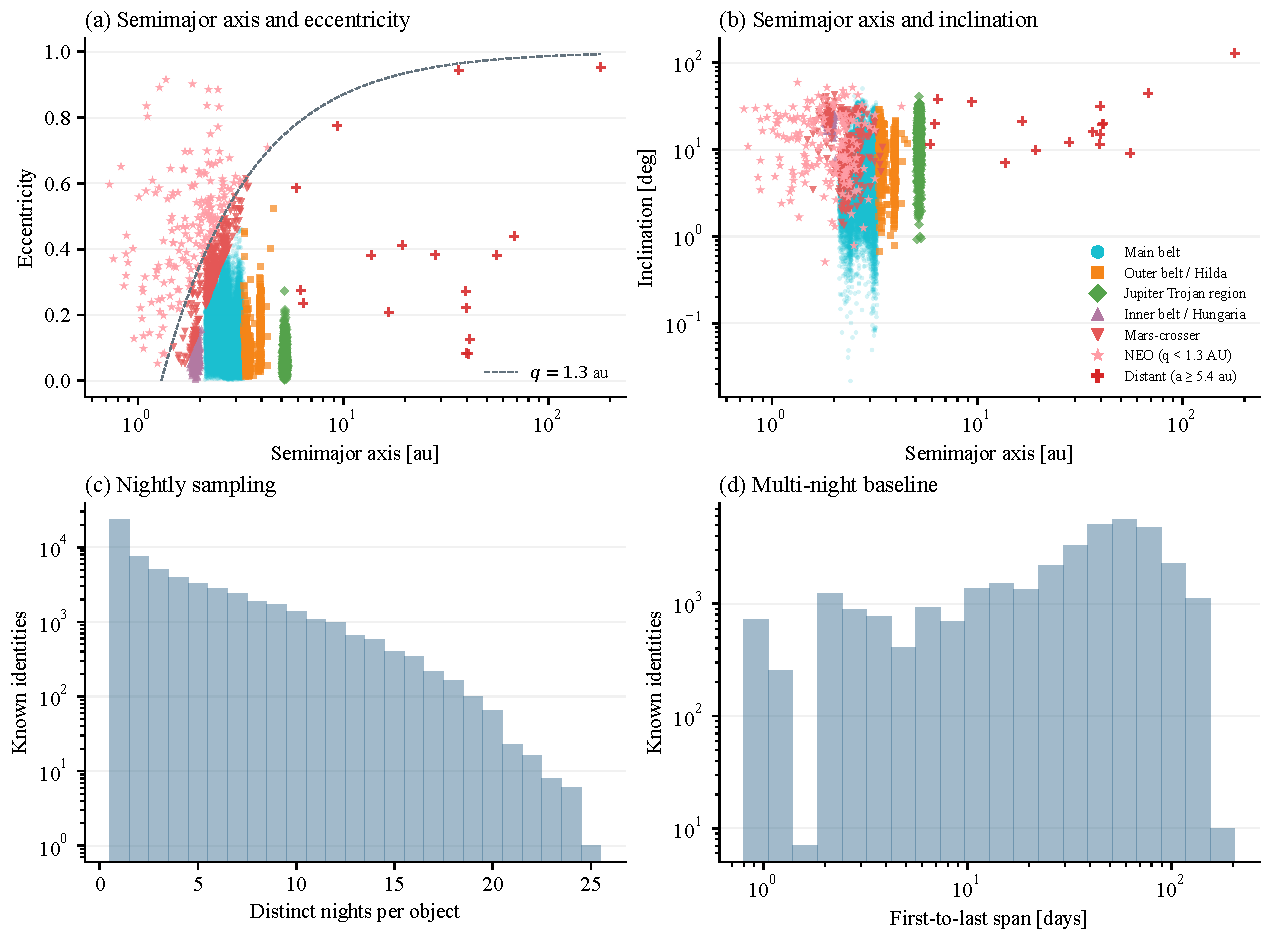
\includegraphics[width=0.98\linewidth]{fig07_orbits_and_revisits.pdf}
\caption{The associated known-object sample, counted once
per catalog identity. (a,b) Archived catalog semimajor
axis versus eccentricity and inclination. Colors and
symbols mark the adopted orbital regions; the dashed
curve in (a) is $q=1.3$~au. The Jupiter Trojan region
is a semimajor-axis selection. Distant-region points retain the 17 catalog identities in the
positional-association sample. Local checks support motion for seven
identities, identify stationary-source coincidences for seven, and leave
three without sufficient evidence.
(c) Number of distinct physical observing nights per
identity. (d) First-to-last measurement span for the
multi-night subset. The vertical count scales in
(c,d) and the semimajor-axis scales in (a,b) are
logarithmic.}
\label{fig:orbits}
\end{figure}

The viewing geometry is predominantly at large solar
elongation. Using target and solar directions from the
same observatory origin, the detection-weighted median
elongation of the validated association sample is
$149.34^\circ$, and its minimum is $59.72^\circ$.
The median measured angular rate of adjacent
within-night association pairs is
26.84~\rateunit. The calculation and distributions
are given in Appendix~\ref{app:checks}. The known-object
branch does not apply the independent search's
$3$--$63$~\rateunit\ window and therefore also records
faster known objects.

\subsection{Historical single-night candidates}
\label{sec:candidates}

The historical independent search produced 4,762
automatic single-night links. Their 14,299 membership
rows correspond to 14,159 unique detection keys because
a detection can occur in more than one proposed link.
Visual review initially marked 68 links as real; 67
were selected for submission, and subsequent image
review retained 58 links containing 179 measurements
on 34 nights (Table~\ref{tab:candidates}). All 179 measurements
map to validated exposures, and every retained linkage contains at
least three distinct exposures within one physical observing night.
The reviewed sample is therefore unchanged by exposure validation;
the automatic catalog and review stages retain the selection of
the original search.

\begin{table}[tbp]
\centering
\caption{Historical Single-Night Candidate Record}
\label{tab:candidates}
\begin{tabular}{lr}
\toprule
Stage & Number of links\\
\midrule
Automatic catalog & 4,762\\
Initially marked real in image review & 68\\
Selected for submission & 67\\
Retained after subsequent image review & 58\\
\quad Consistent with C/2025~Y1 in ephemeris checks & 6\\
\quad Identity unresolved in the frozen analysis & 52\\
\bottomrule
\end{tabular}
\tablecomments{The retained sample comprises 179
measurements on 34 nights, all in validated exposures. Links are single-night
measurement groupings; the entries are not counts
of independently identified new objects.}
\end{table}

Figure~\ref{fig:candidate} presents a retained
three-image sequence from 2026 February~10. The
midpoint times span approximately 79~min, and the
measured linear sky-plane rate is
61.34~\rateunit, close to the upper edge of the
historical search window. The sequence illustrates
the direct image evidence behind an individual
linkage. Appendix~\ref{app:shortarc} shows the arc
spans and short-arc residuals for the retained
sample.

\begin{figure}[tbp]
\centering
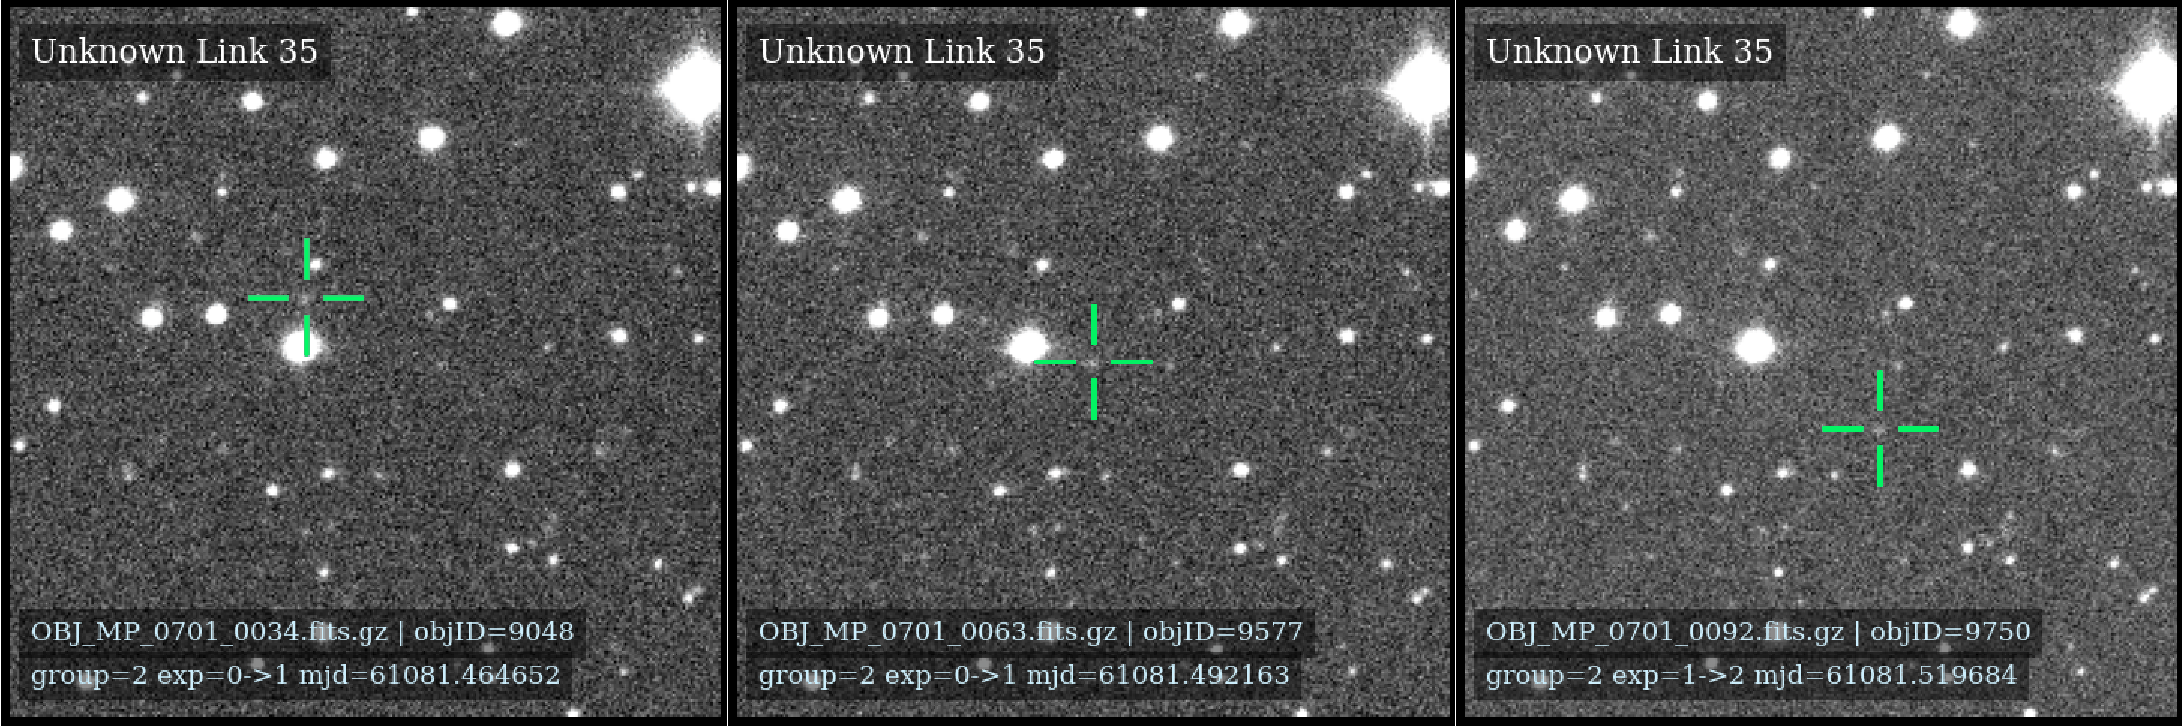
\includegraphics[width=\linewidth]{fig08_candidate.pdf}
\caption{The three original frames of the retained
2026 February~10 linkage 35, with historical
identifier \texttt{00000P2}. The panels are ordered
from left to right at UTC exposure midpoints
11:09:05.959, 11:48:42.908, and 12:28:20.720.
The green marker identifies the detection in each
frame. The fitted linear rate is approximately
61.34~\rateunit. This sequence is an example
of an image-reviewed single-night linkage.}
\label{fig:candidate}
\end{figure}

Two sets of archived ephemeris comparisons support
the numerical association of six retained links
with C/2025~Y1 (ATLAS). The comet remained in the
candidate stream because the contemporaneous
known-object prediction catalog contained asteroid
orbits. The other 52 links have unresolved
identities at the frozen analysis epoch. Their
measured positions, times, brightnesses, and
angular motion are the observational result;
authoritative identity reconciliation and
cross-night association would establish how
many physical objects they represent.

\FloatBarrier
\section{Transient Sources}
\label{sec:transients}

\section{Discussion}
\label{sec:discussion}


The initial campaign establishes \SHARP\ as a
wide-area source of repeated main-belt asteroid
measurements. The population represented by the
primary associations, together with the observed
elongation distribution, locates the survey's
current scientific emphasis. Its most immediate
contribution is additional astrometric and
photometric sampling of cataloged asteroids
over a broad ecliptic region.

The footprint and cadence characterize
complementary aspects of that contribution.
Nearly all of the accumulated geometric
footprint received three exposures within a
single night at some point in the campaign,
whereas only 67.43\% of individual
field--night pointing groups supplied at
least three validated visits. Reaching a
field on one well-sampled night does not
ensure a complete sequence whenever the
field is revisited. Completion of repeated
visits is therefore an important factor in
the area available for constructing
trajectories on a particular night.

At the median adjacent-visit interval of
37.65~min, the historical search window
corresponds to a displacement of approximately
$1.9$--$39.5\asec$. At the slow end,
adjacent-visit displacements are only
a few arcseconds, making the treatment
of stationary-source matches and
small-displacement pairs particularly
relevant. The reduced conditional retention
at $3$--$5$~\rateunit\ identifies a part of
the detected input sample for which the
stored processing is less effective, although
the present aggregate test does not isolate
the responsible processing stage.


The known-object sample combines more than
half a million positional associations with
calibrated aperture photometry. Its
object-level revisit distributions provide
the information needed to select targets
with useful time coverage. The median
four measurements on two nights describes
sparse sampling for a typical identity,
while the more frequently observed objects
offer longer sequences for subsequent
analysis. Rotational studies will require
object-by-object assessment of phase
coverage, blending, changing observing
geometry, and the photometric passband
\citep{WarnerHarrisPravec2009}.

The measured photometric repeatability
and astrometric residuals support
using these catalogs to construct
selected time series with documented
uncertainties. Cadence remains an
equally important constraint: completing
three visits supplies a within-night
trajectory, whereas observations spread
across additional nights extend the
astrometric arc and the range of
rotational phases sampled.

Population-level applications will
also require a selection function.
The conditional retention test
describes linking after catalog
detection. A total selection function
would additionally need the
probability of obtaining a catalog
detection and a usable sequence
for each source and observing
condition.


The retained candidate sample supplies
positions, angular motion, and brightness
over observed single-night arcs. The
short-arc fits establish a consistency
check, but longer baselines are needed
to constrain the poorly determined
line-of-sight motion and obtain secure
identities \citep{Kubica2007,Holman2018,Moeyens2021}.
Connecting existing detections across
nights and obtaining timely follow-up
would therefore add physical information
to the single-night sample.

The C/2025~Y1 example also shows how the
contents of the reference orbit catalog
affect the interpretation of a residual
moving-source stream. Maintaining
asteroid and comet attribution as
explicit steps will allow future
searches to distinguish catalog coverage
from unexplained motion. The initial
results provide concrete trajectories
on which those developments can be
evaluated.

\section{Conclusions}
\label{sec:conclusions}

We have presented the design and initial
observing performance of the \SHARP\
ecliptic survey with the Xinglong
60/90~cm Schmidt telescope. The
validated 2025 November--2026 July
sample contains 39,590 exposures on
129 observing nights, corresponding
to 329.95~hr of open-shutter time.
Its geometric footprint covers
$10,928.1~\degsq$, of which
$10,470.6~\degsq$ received at least
three exposures within a single
night during the campaign. The
median adjacent-visit interval is
37.65~min, and the median span of
sequences with at least three
visits is 78.23~min.

The median catalog $5\sigma$ model
depth is 20.25~mag on the adopted
white-light scale. Selected
within-night stellar sequences
provide a direct repeatability
check on the photometry. The
primary $1\asec$ association
sample contains 531,612
measurements of 58,281 catalog
identities and has a median
radial O$-$C of $0.263\asec$.
Approximately 96\% of the
identities lie in the main-belt
orbital region.

The frozen historical processing
retains 74.16\% of eligible,
already-detected known-object
nights in a retrospective
linkage assessment; applying the validated exposure selection gives
a consistent 74.14\%. Image review retains 58
single-night candidate links,
six numerically consistent with C/2025~Y1. All 179 measurements in these
links belong to validated exposures. These results
define the initial scope of
\SHARP: repeated wide-area
ecliptic imaging that supplies
asteroid positions and
photometry, with a motion
search characterized in
relation to its observed
cadence. They provide the
basis for subsequent asteroid
time series, cross-night
association, and targeted
follow-up.

\section*{Data and Software Availability}

The frozen measurements, exposure ledger, summary tables, and analysis
scripts are available in the SHARP repository.\footnote{\url{https://github.com/xiaoyunao/SHARP/tree/2f5f71d5a074c4cfd712b0e3fbef240c40745e2a/paper_revision_20261015}}
The analysis release is pinned to commit \texttt{2f5f71d5}; its
manifest records the scientific inputs and their provenance. The
historical moving-object configuration is identified by commit
\texttt{d2f0057}. The plotting data and scripts for the revised
Figures~\ref{fig:workflow}, \ref{fig:quality}, and \ref{fig:retention}
also accompany this manuscript.

% Authors, affiliations, contributions, facilities, funding, and
% acknowledgments will be finalized by the authors before submission.

\FloatBarrier
\appendix
\setcounter{figure}{0}
\renewcommand{\thefigure}{A\arabic{figure}}
\renewcommand{\theHfigure}{A.\arabic{figure}}
\renewcommand{\theHequation}{A.\arabic{equation}}
\section{Viewing Geometry and Short-Arc Checks}
\label{app:checks}

\subsection{Solar elongation and angular rate}
\label{app:geometry}

Solar elongation is evaluated using target and
solar directions with a common observing
origin. The archived ALEPH calculation
subtracts the observer's heliocentric
position from the light-time-corrected
heliocentric asteroid position in
J2000-equatorial axes. In that same
representation, let $\boldsymbol{r}_{\rm o}$
be the observer vector and
$\boldsymbol{r}_{\rm a}(t-\tau)$ the
retarded asteroid vector. The unit
directions and elongation are
\begin{align}
\hat{\boldsymbol{u}}_{\rm a} &=
\frac{\boldsymbol{r}_{\rm a}(t-\tau)-\boldsymbol{r}_{\rm o}(t)}
 {|\boldsymbol{r}_{\rm a}(t-\tau)-\boldsymbol{r}_{\rm o}(t)|},\\
\hat{\boldsymbol{u}}_\odot &=
-\frac{\boldsymbol{r}_{\rm o}(t)}{|\boldsymbol{r}_{\rm o}(t)|},\\
\epsilon &= \cos^{-1}
  \left(\hat{\boldsymbol{u}}_{\rm a}\cdot
        \hat{\boldsymbol{u}}_\odot\right).
\end{align}
An independent calculation from the
archived DE432s Sun, Earth, and site
vectors agrees within $0.009\asec$
over the frozen matched epochs.

For the 531,612 primary associations
in validated exposures, the median
elongation is $149.34^\circ$. The
minimum, $59.72^\circ$, occurs for
(1520)~Imatra at 2026 January~26
10:35:38.531~UTC. At that epoch the
geometric solar and target altitudes
are approximately $-14.45^\circ$
and $+43.88^\circ$, respectively.
The elongation distribution in
Figure~\ref{fig:geometry} is weighted
by individual associations.

Angular rates instead use adjacent
pairs of associations belonging
to the same identity and physical
observing night, with different
exposures and a positive time
interval. We divide the great-circle
separation by that interval,
calculating rates separately from
predicted and measured positions.
There are 304,909 valid pairs,
with median predicted and measured
rates of 26.84 and
26.84~\rateunit\ after rounding.
The five pairs above
1,000~\rateunit\ belong to
2026~AA and 2026~CA and have
consistent predicted and observed
displacements. They are retained
as real fast-motion examples
within the known-association
sample.

\begin{figure}[tbp]
\centering
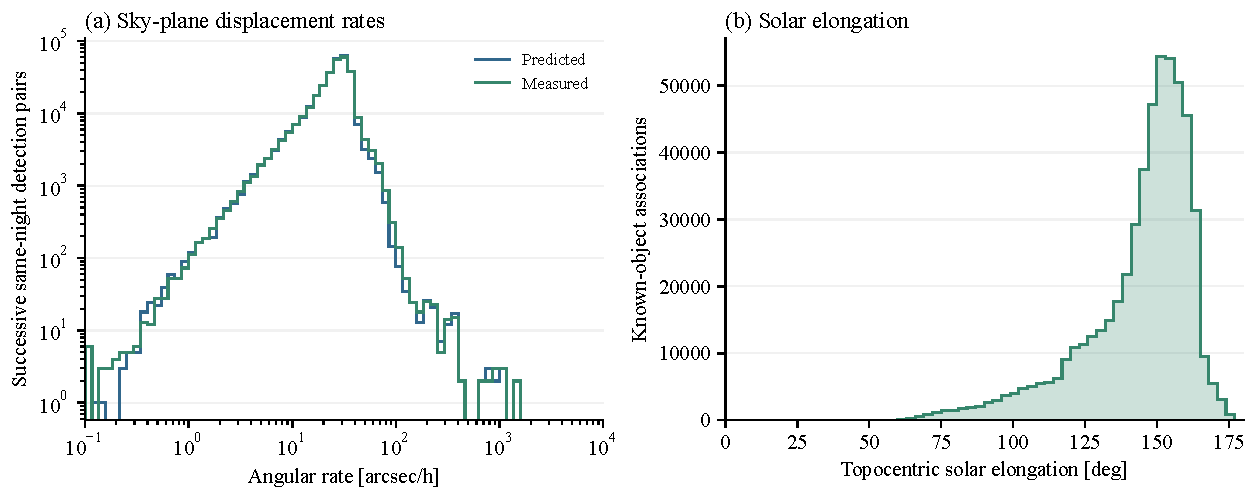
\includegraphics[width=\linewidth]{figA1_motion_and_solar_elongation.pdf}
\caption{Viewing geometry and angular
motion. The rate distributions use
304,909 adjacent within-night pairs
of distinct exposures for the same
known identity; predicted and
measured rates are calculated
separately from great-circle
separations. The elongation
distribution uses the 531,612
validated primary associations,
counting every association and
using the same observing origin
for the Sun and target.
The known-object sample is
not restricted to the
$3$--$63$~\rateunit\ interval
used by the independent
motion search.}
\label{fig:geometry}
\end{figure}

\subsection{Candidate timing and fit diagnostics}
\label{app:shortarc}

The historical short-arc calculation uses
equal endpoint heliocentric-distance
hypotheses with zero assumed radial
derivatives to construct the endpoints;
it does not continuously optimize
the two line-of-sight ranges.
The provisional tracklet-subset
search permits seeds with final-epoch
heliocentric speeds below
140~km~s$^{-1}$. The subsequent
refit returns to the
35~km~s$^{-1}$ acceptance limit
specified in
Section~\ref{sec:motion_method}.

Figure~\ref{fig:shortarc} compares
the exposure-midpoint span and
short-arc fit RMS of the 58
retained historical linkages.
The six links consistent with
C/2025~Y1 are marked separately.
The RMS summarizes internal
agreement over the observed
short arc; a small value with
only a few measurements does
not establish a unique
heliocentric orbit.

The original tracklet, link,
and orbit calculations used
exposure midpoints. The
historical unknown-candidate
ADES export instead wrote
exposure-start times. The
paper's 179-measurement table
uses the original exposure
duration to correct each
exported epoch to its
midpoint. The median offset
is $+15.0015$~s, corresponding
to a median along-track
displacement of $0.0617\asec$
and a maximum of
$0.2556\asec$ at the
measured rates. This
correction concerns the
reported measurement times;
it does not alter the
epochs used to construct
the original linkages.

The historical short-arc
implementation adopted the
same longitude as the
known matcher but latitude
$40.394239^\circ$ and
height 868.221~m. A
128-night sensitivity
comparison between these
two site specifications
found no change in the
stored fit-success or
diagnostic-quality
classification. The
as-executed coordinates
and the comparison are
preserved with the
analysis products.

\begin{figure}[tbp]
\centering
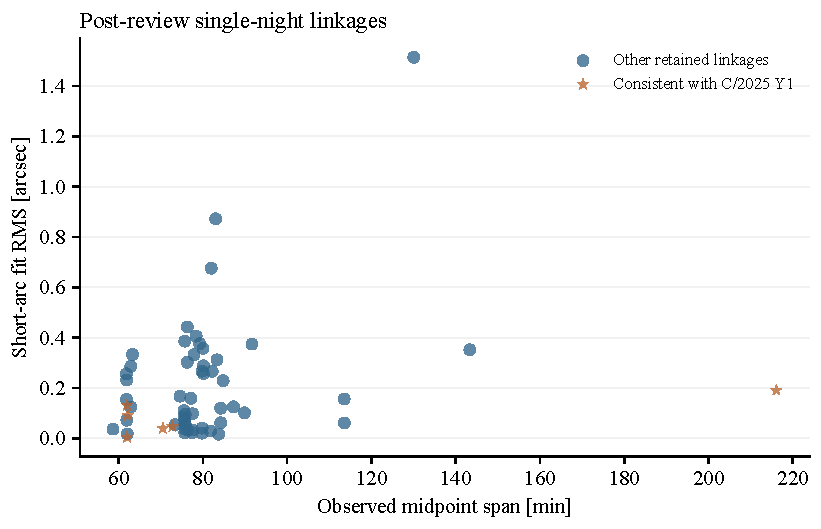
\includegraphics[width=0.75\linewidth]{figA2_candidate_short_arc_diagnostic.pdf}
\caption{Exposure-midpoint span and
short-arc fit RMS for the
58 image-reviewed historical
single-night linkages.
The six numerically
associated with C/2025~Y1
are shown separately.
These values describe
within-arc consistency,
rather than uncertainties
of uniquely determined
orbits.}
\label{fig:shortarc}
\end{figure}

\FloatBarrier
\bibliography{references}
\bibliographystyle{aasjournalv7}
\end{document}
